\documentclass[a4paper]{article}

\usepackage{amsmath}
\usepackage{physics}
\usepackage{hyperref}
\usepackage[all]{hypcap} % Make a hyperlink navigate to the top of the figure
\usepackage{graphicx}
\graphicspath{ {./images/} }
\usepackage[a4paper,left=3cm,right=3cm,top=2.5cm,bottom=2.5cm]{geometry}

\title{Quantum Phase Estimation}
\author{Tzu Hsuan Chang}

\begin{document}
\maketitle

\section{Introduction}
\label{sec:Intro}
Quantum phase estimation (QPE) is used to find the eigenvalues of a unitary matrix. Suppose we want to find the eigenvalues $e^{2 \pi i \theta_i}$ corresponding to the eigenvector $\ket {u_i}$ of an unitary operator $\hat{U}$ such that
$\hat{U} \ket{u_i}  = e^{2 \pi i \theta_i} \ket{u_i}$. The QPE have the following operation,
    \begin{equation} \label{eq:eq1}
    \setlength{\jot}{10pt}
        \ket{0} \ket{u_i}   \longrightarrow   \ket{\tilde \theta_i} \ket{u_i},
    \end{equation}
where $\tilde \theta_i$ is an estimate for $\theta_i$.

As shown on figure~\ref{fig:qpe}, the QPE circuit write the phase of $\hat U$ to n ancillary qubits $\ket{0}^{\otimes n}$ in the Fourier basis and using inverse QFT to transform them back to the computational basis. The following is the mathematical details.

\subsection*{Mathematical details}
\label {subsec:qpe}

As shown in figure~\ref{fig:qpe}, assuming $\psi$ is the eigenvector of the unitary operator $\hat U$ with eigenvalue $e^{2 \pi i \theta}$. Initially, we have
    \begin{equation} \label{eq:eq2}
    \setlength{\jot}{10pt}
        \psi_0 = \ket{0}^{\otimes n} \psi.
    \end{equation}
After applying n-bit Hadamard gates on the ancillary qubits,
    \begin{equation} \label{eq:eq2}
    \setlength{\jot}{10pt}
        \psi_1 = \frac{1}{2^{n/2}} (\ket{0} + \ket{1})^{\otimes n} \psi.
    \end{equation}

    \begin{figure}
        \centering
            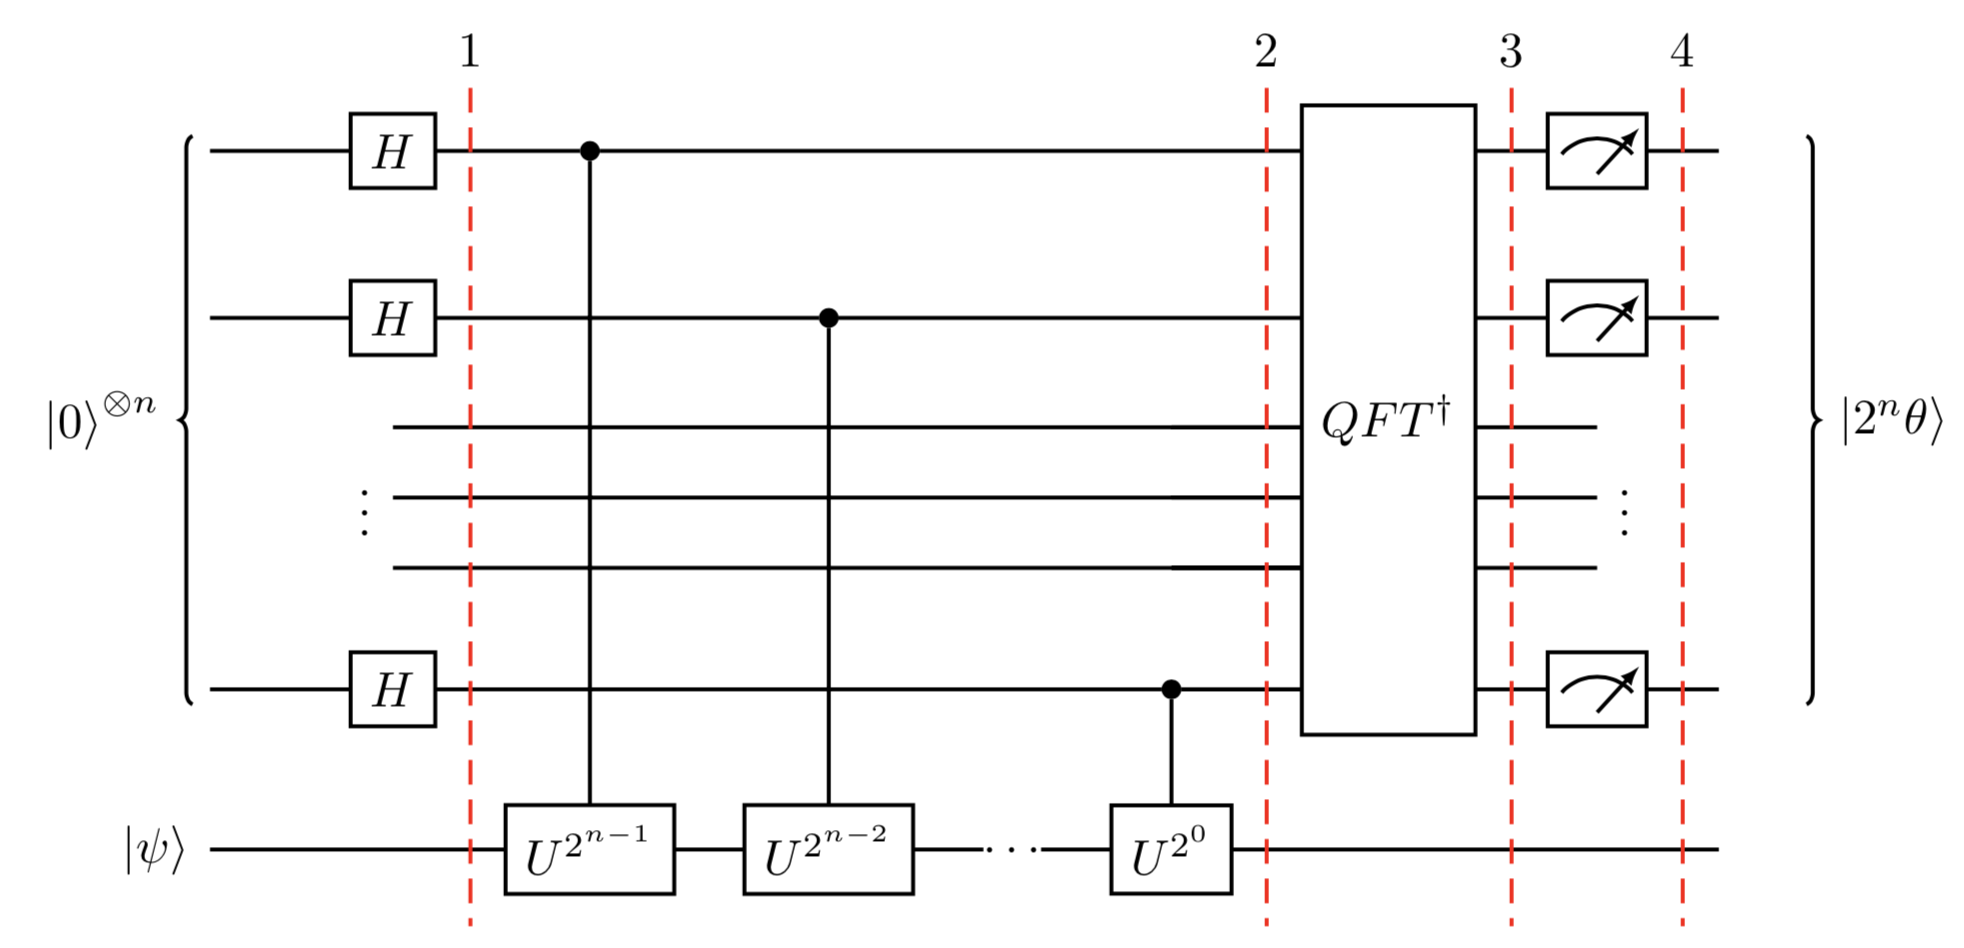
\includegraphics [width=\textwidth, height=\textheight, keepaspectratio] {qpe_tex_qz.png}
        \caption{Quantum phase estimation circuit.\cite{Qiskit-Textbook}}
        \label{fig:qpe}
    \end{figure}


\bibliographystyle{abbrv}
\bibliography{references}

\end{document}